\documentclass[runningheads]{llncs}

\usepackage{graphicx}
\usepackage{indentfirst}
\usepackage{hyperref}
\usepackage{algorithm}
\usepackage[noend]{algpseudocode}

\setcounter{secnumdepth}{3}

\begin{document}

% \thanks{Supported by organization x.}
\title{Parallel Genetic Algorithm for Regression}

\author{Paulo Santos \and
Maria Fidalgo
}
%\authorrunning{F. Author et al.}

\institute{Departamento de Informática da Faculdade de Ciências da Universidade de Lisboa
\email{\{fc47806,fc49034\}@alunos.fc.ul.pt}}

\maketitle

\begin{abstract}
The first sentence of an abstract should clearly introduce the topic of the paper so that readers can relate it to other work they are familiar with. However, an analysis of abstracts across a range of fields show that few follow this advice, nor do they take the opportunity to summarize previous work in their second sentence. A central issue is the lack of structure in standard advice on abstract writing, so most authors don’t realize the third sentence should point out the deficiencies of this existing research. To solve this problem, we describe a technique that structures the entire abstract around a set of six sentences, each of which has a specific role, so that by the end of the first four sentences you have introduced the idea fully. This structure then allows you to use the fifth sentence to elaborate a little on the research, explain how it works, and talk about the various ways that you have applied it, for example to teach generations of new graduate students how to write clearly. This technique is helpful because it clarifies your thinking and leads to a final sentence that summarizes why your research matters.

\keywords{Parallel Genetic Programming \and Regression \and Island Model.}
\end{abstract}


%%%%%%%%%%%%%%%%%%%%%%%%%%%%%%%%%%%%%%%%%%%%%%%%%%%%%%%%%
%%%%%%%%%%%%%%%%%%%%%%%%%%%%%%%%%%%%%%%%%%%%%%%%%%%%%%%%%
\section{Introduction}

Genetic Algorithms (GAs) are metaheuristic searching algorithms where the main idea lies in following the same principles as Natural Selection and Evolution in Biology \cite{sivanandam2008genetic}. That is, the algorithms work around a \textit{population} of potential solutions for the problem, the \textit{individuals}. The population changes during the execution of the algorithm, mimicking the evolution of a real population of living beings, from generation to generation, where the fitter individuals are more likely to survive and reproduce.

The algorithm is composed by three main operations: Fitness, Crossover and Mutation. Fitness measures how good an individual is; Crossover (or sexual reproduction) generates a new solution based on two existing ones, simulating the breeding of two individuals; and Mutation (or asexual reproduction) produces random changes to an individual \cite{langdon1995genetic}.

Due to the characteristics of the GAs, applications are often related to optimization \cite{sivanandam2008genetic}, such as the Traveling Salesman Problem \cite{grefenstette1985genetic}, classification \cite{5340522}, decision making \cite{George:2012:GAB:2345396.2345426} and prediction \cite{etemadi2009genetic}.

Prediction can be accomplished through Regression Analysis, which is the task of modeling a random variable $Y$ as a function of a vector of random variables $X$. This may be translated as the task of finding the mathematical expression best suited to explain $Y$. Regression models presuppose the existence of constants, called \textit{parameters}, that are to be estimated from the data \cite{rawlings2001applied}.

However, when using Genetic Algorithms for this type of problem, it is not the parameters that we want to estimate but the whole mathematical expression. Therefore, we will be looking for the one that minimizes the error between the value provided by the model and the actual value.

In this work, we explore different parallelizations of the Genetic Algorithm for regression, using the toxicity dataset \cite{krawiec2013genetic}. We will start by introducing the algorithm and its operations in further detail. Next, we will present the several approaches studied:

\begin{itemize}
\item Sequential
\item Adaptive Sequential
\item Trivial Parallelization
\item Island Parallelization
\end{itemize}

Finally, we will demonstrate the experimental evaluation and compare with each other.

%%%%%%%%%%%%%%%%%%%%%%%%%%%%%%%%%%%%%%%%%%%%%%%%%%%%%%%%%
%%%%%%%%%%%%%%%%%%%%%%%%%%%%%%%%%%%%%%%%%%%%%%%%%%%%%%%%%
\section{Genetic Algorithm}

\begin{algorithmic}
   \State \textbf{Input}:$Max_{gen},Pop_{size},P_{cross},P_{mut},P_{reproduction}$
   \State \textbf{Output}:$S_{best}$
   \State $Population\gets InitializePopulation(Pop_{size},nodes_{func},nodes_{term})$
   \State $MeasureFitness(Population)$
   \State $S_{best} \gets GetBestSolution(Population)$
   \State $Generation_{i} \gets 0$
   
   \While{$Generation_{i} \not= Max_{gen}$}
      \State $Generation_{i} \gets Generation_{i} + 1$
      \State $NewPopulation \gets \emptyset$
      \State $AddElitesToNewPopulation(Population,NewPopulation)$
   
      \While{$Size(NewPopulation) < Pop_{size}$}
         \State $Ind_{1}, Ind_{2} \gets SelectForCrossover(Population, P_{reproduction})$
         \State $NewGeneration \gets NewGeneration \cup Mutate(Crossover(Ind_{1},Ind_{2},P_{cross}),P_{mut})$
         \State $MeasureFitness(NewPopulation)$
      \EndWhile
      
      \State $S_{best} \gets GetBestSolution(NewPopulation)$
      \State $Population \gets NewPopulation$
   \EndWhile
   \State \textbf{return} $S_{best}$
\end{algorithmic}

\subsection{Fitness}

\subsection{Crossover}

\subsection{Mutation}

%%%%%%%%%%%%%%%%%%%%%%%%%%%%%%%%%%%%%%%%%%%%%%%%%%%%%%%%%
%%%%%%%%%%%%%%%%%%%%%%%%%%%%%%%%%%%%%%%%%%%%%%%%%%%%%%%%%
\section{Approach}



%%%%%%%%%%%%%%%%%%%%%%%%%%%%%%%%%%%%%%%%%%%%%%%%%%%%%%%%%
%%%%%%%%%%%%%%%%%%%%%%%%%%%%%%%%%%%%%%%%%%%%%%%%%%%%%%%%%
\section{Implementation Details}

\subsection{Abstract Syntax Tree}
The implementation of an Abstract Syntax Tree allows us to easily generate random mathematical expressions with an immutable tree where each node either represents a binary operator node or a constant node, which can be a variable or value.

Each tree contains a crossover operation which allows it to generate offspring by crossing itself with another tree in a single-point of crossing. This has been accomplished by randomly choosing and swapping two nodes from each tree.

Every tree may also mutate itself by randomly choosing one node and changing its inner value. A constant binary node could have its inner content changed with a new value or variable, while binary operator nodes would have their operation changed.

As aboved-mentioned, Abstract Syntax Tree allows us to generate random mathematical expressions. By using an expression builder\footnote{\href{https://www.objecthunter.net/exp4j/index.htm}{exp4j - Expression Builder from String for Java}} was possible to set values to variables of a given expression and obtain a result useful to calculate the fitness of the tree.

\subsection{Regular Genetic Algorithm}
The linear implementation of a regular genetic algorithm where each genetic algorithm operation has fixed ratios. 

The fitness is measured using a linear regression \textbf{TODO:} %%%%%%%%%%%%%%%%% MARIA !!! Eu nao sei esta parte do measure fitness com regressao linear

The population is sorted from best fitness to worst fitness using a default arrays sorting algorithm from Java.

The best individual from each generation is remains unchanged to the next generation. The rest of the population is replaced with generated offsprings by crossing parents using a Fitness Proportionate Selection, where the best individuals have a higher chance of being chosen for crossover.

Each offspring contains 10\% chance of being selected to suffer a mutation.

\subsection{Adaptative Genetic Algorithm}
The linear implementation of a genetic algorithm where the mutation crossover rates are adaptative  depending on the progression made by each operation in the last generation \cite{adaptativeCrossOverMutation}. The measure fitness and sorting is implemented the same way has in the Regular Genetic Algorithm.

The best individual still remains from each generation unchanged to the following one. The new offsprings are generated by crossing parents using an Adapted Fitness Proportionate Selection. Since new offsprings are always generated by crossing two individuals, the crossover rate will influence the probability each individual has to be chosen. This has been attained by using the absolute value of  normal probability density function and multiplying it by the sum of a third of the amount of population with the crossover rate. The crossover rate is an integer value between \(-populationSize\) and \(populationSize\).

\[ \left |\left | \frac{1}{\sigma \sqrt{2\pi}}*e^{-\frac{(-\mu)^2}{2\sigma^2}} \right | * (popSize\,/\,3) + crossoverRate)  \right | \%  \, popSize \]	

The mutation rate controls the probability of an individual to suffer a mutation. This value is a value between 0.05 and 1.0.

Both of these rates are updated according to the progressions they obtained for each individual. The chosen mutation rate offset is 0.05 and the crossover rate offset is \(populationSize * 0.025\).

\begin{algorithmic}
\If {$mutationProgress < crossOverProgress$}
        \State $mutationRate \gets min(1.0, mutationRate + mutationOffset)$
        \State $crossoverRate \gets max(-popSize, crossoverRate - mutationOffset)$
\EndIf
\If {$mutationProgress > crossOverProgress$}
        \State $mutationRate \gets max(mutationOffset, mutationRate - mutationOffset)$
        \State $crossoverRate \gets min(popSize, crossoverRate + mutationOffset)$
\EndIf
\end{algorithmic}

\subsection{Parallel Versions Implementation}
\subsubsection{Parallel Population Sorting} \hfill \par
Due to parallel mergesort ease of implementation and advantages of execution time \cite{analysisMergeSort}, the sorting of the population by fitness has been implemented with a parallel mergesort with linear insertion sort when the amount of population to compute is smaller than an offset of 7. The population is splitten by half until the offset is reached and the insertion sort and merge algorithms' are computed.


\subsubsection{ForkJoin} \hfill \par
\textbf{TODO:}

\subsubsection{Phaser} \hfill \par

\subsubsection{Island}

%%%%%%%%%%%%%%%%%%%%%%%%%%%%%%%%%%%%%%%%%%%%%%%%%%%%%%%%%
%%%%%%%%%%%%%%%%%%%%%%%%%%%%%%%%%%%%%%%%%%%%%%%%%%%%%%%%%
\section{Evaluation}

\subsection{Experimental Setup}
\textbf{TODO:} \\
24 cores, \\ 1000 pop,\\  500 iteracoes, \\ 
tamanho geracao inicial \(2^{10}\), \\ 
tamanho maximo com crossover \(2^{15}\) \\
dataset offset = 250 iteracoes. \\
dataset split = 100 = 2 partes. \\

In this section you should describe the machine(s) in which you are going to evaluate your system. Select the information that is relevant.


\subsection{Results}

+ Comparacao dos resultados da regular linear com a adaptative linear

+ Comparacao dos resultados da de ilhas com 6 ilhas, 12 ilhas, 18 ilhas e 24 ilhas

+ Comparacao de todas as implementacoes em termos finais de execucao com boxplot

+ Apresentacao em linha de tempo da linear, forkjoin e phaser

+ Comparacao em linha de tempo da linear, forkjoin, phaser, ilhas com 6

In this section you should present the results. Do not forget to explain where the data came from. 

You should include (ideally vectorial) plots, with a descriptive caption. Make sure all the plots (Like Figure~\ref{fig1} are well identified and axis and metrics are defined.

%\begin{figure}[htbp]
%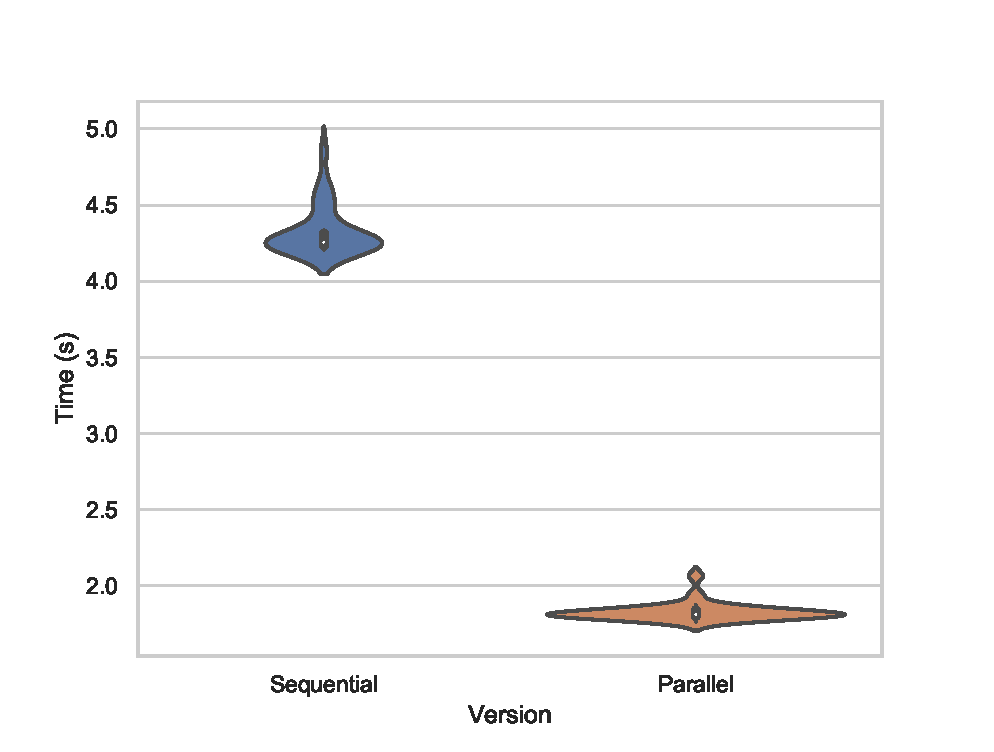
\includegraphics[width=\textwidth]{code/performance.eps}
%\caption{Comparison of the performance of sequential and parallel versions of the algorithm.} \label{fig1}
%\end{figure}


\subsection{Discussion}

Here you should discuss the results on a high level. For instance, based on our results, the parallelization of the merge-sort is relevant as no other parallel work occurs at the same time, and the complexity $O(N log(N))$ can have a large impact when the number of individuals is high.

%%%%%%%%%%%%%%%%%%%%%%%%%%%%%%%%%%%%%%%%%%%%%%%%%%%%%%%%%
%%%%%%%%%%%%%%%%%%%%%%%%%%%%%%%%%%%%%%%%%%%%%%%%%%%%%%%%%
\section{Related Work}

Several implementations of the genetic algorithm were made throughout the years. We will shortly talk about two implementations and how they fit in the scope of our work.

Dominic and Willis  \cite{GPTIPS} developed a MATLAB toolbox, GPTIPS, which is able to perform regression through genetic programming. The main difference between their approach and  ours is that they do not explore the parallelism of the algorithm, focusing on the usability of the toolbox. Moreover, they chose to include nonlinear operators, that we decided to leave out. Our work is, therefore, important to whom intends to develop a fast approach of the genetic classifier. Additionally, GPTIPS requires the purchase of a payed software (MATLAB), available to a less broader population.

Jenetics \cite{jenetics} is another genetic programming implementation. It is a Java library designed to abstract different concepts within the genetic programming panorama, such as Gene, Genotype and Chromosome, allowing it to serve a vast spectrum of domains. This library implements the Java Stream Interface and provides ForkJoin Parallelization. This is, therefore, a generic purpose implementation for genetic algorithm. On the other hand, in our work we provided a study of genetic programming specific for regression, where other parallelization techniques were able to achieve better results than ForkJoin, like the Island Models.

%%%%%%%%%%%%%%%%%%%%%%%%%%%%%%%%%%%%%%%%%%%%%%%%%%%%%%%%%
%%%%%%%%%%%%%%%%%%%%%%%%%%%%%%%%%%%%%%%%%%%%%%%%%%%%%%%%%
\section{Conclusions}

Here you should resume the major conclusions taken from discussion. Ideally, these should align with the objectives introduced in the introduction.


You should also list the future work, i. e., tasks and challenges that were outside your scope, but are relevant.

%%%%%%%%%%%%%%%%%%%%%%%%%%%%%%%%%%%%%%%%%%%%%%%%%%%%%%%%%
%%%%%%%%%%%%%%%%%%%%%%%%%%%%%%%%%%%%%%%%%%%%%%%%%%%%%%%%%
\section*{Acknowledgements}

First Author wrote the part of the program implemented the phasers. Second Author implemented the MergeSort in parallel. 

Both authors wrote this paper, with First Author focusing on the introduction, related work and conclusions while the Second Author focused on approach and evaluation.

Each author spent around 30 hours on this project.

\bibliographystyle{splncs04}
\bibliography{bibliography}

\end{document}
